% !TeX document-id = {c68ea1ac-ebac-4541-a297-17005c6d2297}
% !TeX encoding = UTF-8
% !TeX spellcheck = en_US
% !TeX TS-program = pdflatex
% !TeX TXS-program:bibliography = biber -l zh__pinyin --output-safechars %

\documentclass[
	10pt
%	,draft
%	,handout
	,noamsthm
]{beamer}

% to be `\input` in subfolders,
% ... therefore the path should be relative to subfolders.

\usepackage{iftex}
\ifPDFTeX
\else
	\usepackage[UTF8
		,heading=false
		,scheme=plain % English Document
	]{ctex}
\fi
%\ctexset{autoindent=true}
\usepackage{indentfirst}

\input{../.modules/basics/macros.tex}
\input{../.modules/preamble_base.tex}
\input{../.modules/preamble_beamer.tex}
\input{../.modules/basics/biblatex.tex}


%Misc
	\usepackage{lilyglyphs}
	\newcommand{\indicator}{$\text{\clefG}$}
	\newcommand{\indicatorInline}{$\text{\clefGInline}$}

\newcommand{\legacyReference}{{
%	\clearpage\par
%	\quad\clearpage
	\def{\midquote}{\textbf{PAST WORK, AS TEMPLATE}}
	\newparagraph
}}

% Settings
\counterwithout{equation}{section}
\mathtoolsset{showonlyrefs=false}
%\DeclareTextFontCommand{\textbf}{\sffamily}

% Spacing
\geometry{footnotesep=2\baselineskip} % pre footnote split
\setlength{\parskip}{.5\baselineskip}
\renewcommand{\baselinestretch}{1.15}


%% List
%	\setlist*{
%		listparindent=\parindent
%		,labelindent=\parindent
%		,parsep=\parskip
%		,itemsep=1.2\parskip
%	}


\addtobeamertemplate{navigation symbols}{}{%
    \usebeamerfont{footline}%
%    \usebeamercolor[fg]{footline}%
    \hspace{1em}%
    \normalsize\insertframenumber/\inserttotalframenumber
}

\makeatletter
\setbeamertemplate{headline}
{%
    \begin{beamercolorbox}[wd=\paperwidth,colsep=1.5pt]{upper separation line head}
    \end{beamercolorbox}
    \begin{beamercolorbox}[wd=\paperwidth,ht=2.5ex,dp=1.125ex,%
      leftskip=.3cm,rightskip=.3cm plus1fil]{title in head/foot}
      \usebeamerfont{title in head/foot}\insertshorttitle
    \end{beamercolorbox}
    \begin{beamercolorbox}[wd=\paperwidth,ht=2.5ex,dp=1.125ex,%
      leftskip=.3cm,rightskip=.3cm plus1fil]{section in head/foot}
      \usebeamerfont{section in head/foot}%
      \ifbeamer@tree@showhooks
        \setbox\beamer@tempbox=\hbox{\insertsectionhead}%
        \ifdim\wd\beamer@tempbox>1pt%
          \hskip2pt\raise1.9pt\hbox{\vrule width0.4pt height1.875ex\vrule width 5pt height0.4pt}%
          \hskip1pt%
        \fi%
      \else%  
        \hskip6pt%
      \fi%
      \insertsectionhead
    \end{beamercolorbox}
% Code for subsections removed here
}
\makeatother

\usepackage{tikz}
%\usepackage{snapshot}

\title{Glue-on AdS holography for $T\bar T$-deformed CFTs}
\subtitle{An extended AdS\,/\,\TTbar duality \textit{(beyond infinity)}}
\author{%
	Wen-Xin Lai 
	\texstringonly{\,}\textkai{赖文昕}%
	\texstringonly{
		\textit{\small in collaboration with} \\
			Luis Apolo,
			Peng-Xiang Hao \textkai{郝鹏翔}
			and Wei Song \textkai{宋伟}\\[2ex]
		\sidenote{\arxiv{2303.04836}}%
%		\ submitted to \textit{JHEP}
	}%
}
\institute{\small%
	Yau Mathematical Sciences Center,\\
	Tsinghua\texstringonly{
%		\\\large\ccbyncsajp
	}\\[2ex]
	\today\ @ BIMSA
}
\date{}


\newcommand{\veccol}[1]{\pqty{
	\begin{smallmatrix}
		#1
	\end{smallmatrix}
}}

\addbibresource{glueon-beamer.bib}
%\usepackage{cprotect}

\usepackage{cancel}
\newcommand{\slot}{{\,\bullet}}

\usepackage{xspace}
\newcommand{\TTbar}{\texorpdfstring{\ensuremath{T\bar{T}}}{TTbar}\xspace}

\begin{document}
{%%% TITLEPAGE
\setbeamercolor{title in head/foot}{
		use=palette quaternary
		,fg=palette quaternary.bg
	}
\logo{}
\begin{frame}
%	\titlegraphic{\vspace{2\baselineskip}}
	\titlepage
	\tikz [remember picture,overlay]
	\node at ([
		yshift=-4.6\baselineskip,
		xshift=.25\linewidth
	] current page.center) {
		\begin{minipage}{.5\textwidth}
		\centering
		\includegraphics[height=.33\textheight]{img/smbc-cantor-cropped.png}
		\\[.2ex]
		\footnotesize \url{https://smbc-comics.com/comic/cantor}
		\hspace{-1.5em}
		\end{minipage}
	};
\end{frame}
}%%% TITLEPAGE

\begin{frame}{Outline}
\raggedbottom
\large
\tableofcontents
\end{frame}

\section{\textbf{Warmup:} Pure Einstein gravity in $\mrm{AdS}_3$ / $\mrm{CFT}_2$}

\newcommand{\citeMaldacena}{%
	\textcite{Maldacena:1997re} --- \scriptsize\citetitle{Maldacena:1997re}
}

\newcommand{\stateAdsCft}{
\begin{align*}
	\textrm{Strings on $\mrm{AdS}_{d+1}$ background}
	&\ \equiv\ 
	\textrm{Conformal Field Theory $\mrm{CFT}_{d}$}
\\
	\textrm{\textit{asympt.}~$\mrm{AdS}_{d+1}$ Gravity}
	&\ \equiv\ 
	\textrm{Large $N$ $\mrm{CFT}_{d}$ at \textit{asympt.}~boundary}
\end{align*}
}

\begin{frame}{AdS/CFT --- holography duality}{%
	\citeMaldacena%
}
\vspace{-2.5\baselineskip}
\stateAdsCft
\vspace{-1.8\baselineskip}
\begin{figure}[!h]
	\centering
	\includegraphics[width=.5\linewidth]{img/ads-cft.png}

	\vspace{-.3\baselineskip}
	\caption{$\mrm{AdS}_3/\mrm{CFT}_2$ cartoon}
	
	\vspace*{-.8\baselineskip}
	\scriptsize\ Image courtesy: \textcite{AldegundePWSep22}
\end{figure}
\vspace{-1.3\baselineskip}
\end{frame}

%\begin{equation}
%	R_{\mu\nu} - \frac{1}{2}\,R g_{\mu\nu}
%	+ \Lambda g_{\mu\nu}
%	= 8\pi G_N T_{\mu\nu}^{\textit{matter}},\quad
%	\Lambda < 0
%\label{eq:einstein}
%\end{equation}

\begin{frame}{AdS/CFT --- a model of quantum gravity}{%
	\citeMaldacena
}
\vspace{-2.4\baselineskip}
\stateAdsCft
\vspace{-1.6\baselineskip}
\pause
\begin{itemize}

\item A model of \textsc{quantum gravity}
\item ... originating from \textsc{string theory}
\item ... seemingly \textsc{Universal / ubiquitous}

\pause
\begin{itemize}
	\item Model agnostic: $\mrm{AdS}_5\times S^5$, $\mrm{AdS}_3\times S^3 \times T^4$, symmetric orbifolds, minimal models, ``monsters'', ... \textit{\small Maldacena, Witten, GKP, ABJM, Gaberdiel, and many many more}
	\item Our work: pure Einstein gravity in $\mrm{AdS}_3$ / $\mrm{CFT}_2$ $(d=2)$.
	
\end{itemize}
\end{itemize}
\end{frame}



%%% LaTeX3e!
\NewDocumentCommand{\figAdsCft}{ O{.28} }{
\begin{column}{#1\textwidth}
\begin{figure}[!h]
	\centering
	\includegraphics[width=\linewidth]{img/ads-cft-cleaner.png}

	\vspace{-.01\baselineskip}
	\scriptsize\textcite{AldegundePWSep22}\ \,
\end{figure}
\end{column}
}


\begin{frame}{$\mrm{AdS}_3/\mrm{CFT}_2$ --- gravity trapped in a cylinder}{%
	\textcite{Aharony:1999ti}
}
\begin{columns}
\figAdsCft
\begin{column}{.75\textwidth}
	\begin{itemize}
	\item $\mrm{AdS}_3$ metric, $\rho \sim z^2 \sim r^{-2}$
	\begin{equation}
	\hspace{-2em}
		ds^2 = \ell^2 \frac{d\rho^2}{4 \rho^2} + \pqty{\frac{1}{\rho} g^{(0)}_{ij} + g^{(2)}_{ij} + \rho\thinmspace g^{(4)}_{ij} + \cdots}\, dx^i dx^j \label{fggauge}
	\end{equation}
	
	\vspace{-.5\baselineskip}
	boundary at $\rho \to 0$, $x^{i} \sim \varphi, t$, $i = 1,2$

\pause
	\item Surprisingly the expansion simply terminates at~$\rho\thinmspace g^{(4)}_{ij}$ for pure Einstein gravity! Moreover,
	\begin{equation}
		g^{(4)}_{ij} = \frac{1}{4} g^{(2)}_{ik} g^{(0)\thinmspace kl}_{\phantom{kl}} g^{(2)}_{lj}
	\end{equation}
	\textcite{Fefferman:2007rka,Banados:1998gg}
	\end{itemize}
\end{column}
\end{columns}
\end{frame}

\newcommand{\eqBanados}{
	\begin{equation*}
	\hspace{-2em}
		ds^2 = \ell^2 \bigg( \frac{d\rho^2}{4 \rho^2} + \frac{ \big( du + \rho \, \mathcal {\bar L}(v)\, dv \big) \big( dv + \rho \, \mathcal L(u)\, du \big) }{\rho} \bigg)\ \,
	\end{equation*}
}

\begin{frame}{$\mrm{AdS}_3/\mrm{CFT}_2$ --- simple realization of holography}{%
	\textcite{Banados:1992wn}
}
\begin{columns}
\figAdsCft
\begin{column}{.72\textwidth}
	\begin{itemize}
	\item $\mrm{AdS}_3$ metric for $\rho > 0$, \\
	\textcite{Banados:1998gg}
	\eqBanados
	$g^{(2)} \leadsto \mathcal L(u)$, $\bar{\mathcal L}(v)$: arbitrary periodic functions,\\
	where $u,v = \varphi \mp it$, $du\,dv = d\varphi^2 + dt^2$
%	\vspace{-.5\baselineskip}
	
\pause
	\item A consequence of Einstein equations \\
	in $(2+1)$ dimensions.\\
	\textit{Too many constraints, too little freedom!}
	\end{itemize}
\end{column}
\end{columns}
\end{frame}


\begin{frame}{$\mrm{AdS}_3/\mrm{CFT}_2$ --- simple realization of holography}{%
	\textcite{Aharony:1999ti}
}
\begin{columns}
\figAdsCft
\begin{column}{.72\textwidth}
	\begin{itemize}
	\item Different \textbf{geometries} in the ``bulk''
	\eqBanados
	specified by $\mathcal L(u)$, $\bar{\mathcal L}(v)$: periodic functions, maps to different \textbf{states} in the boundary $\mrm{CFT}_2$ with stress energy $\ave{T(u)}_\psi$, $\ave{\bar{T}(v)}_\psi$

	\item \textit{Dictionary:} bulk $\leftrightarrow$ boundary quantities:\\
		\begin{itemize}
		\item spectrum,
			symmetry,\\
			partition functions,
			correlators, ...
		\end{itemize}
	\end{itemize}

\end{column}
\end{columns}
\end{frame}

\section{\textbf{Review:} \TTbar deformation and cutoff AdS} \label{se:cutoffholography}

\begin{frame}{\TTbar deformations --- motivations}{%
	Comments taken from \textcite{Cui:2023jrb}
}
\begin{columns}
\figAdsCft
\begin{column}{.72\textwidth}
	\begin{itemize}
	\item Ideally: AdS/CFT
	\item Reality: non-AdS space and non-CFT
	\begin{itemize}
		\item possible to extend holographic principle to more general context?
		\item attempt: \textbf{\textit{deformations}} on both sides\\
		in a controllable way
	\end{itemize}
	\end{itemize}
\end{column}
\end{columns}
\end{frame}

\newcommand{\citeTTbar}{%
	\textcite{Zamolodchikov:2004ce}, revived by \textcite{Smirnov:2016lqw} and \textcite{Cavaglia:2016oda} \textit{et al}
}


\begin{frame}{\TTbar deformations --- definition}{%
	\citeTTbar
}
\begin{itemize}

\item Define ``\,\TTbar\,'' as the flow of action:
\begin{equation}
	\partial_{\sidenote{\mu}} I = -{8 \pi} \int d^2x \, T\bar T =  -{\pi} \int d^2x\,\big( T^{ij}T_{ij}- (T^i_i)^2 \big)
	\label{TTbardef}
\end{equation}
For $\mrm{CFT}_2$,\ $T\bar{T} = T_{xx} T_{\bar{x}\bar{x}}$,\ where $x, \bar{x} = \varphi' \mp it'$.

\item The stress tensor $T_{ij}(\sidenote{\mu})$ on the right hand side flows with the deformation parametrized by $\sidenote{\mu}$. 

\pause

\item This is thus a \textit{differential equation} for a flow, starting from some generic QFT specified by $I(\mu = 0)$. In this work we shall start from $\mrm{CFT}_2$, but note that \TTbar is \textit{irrelevant}: conformal symmetry will be broken.

\end{itemize}
\end{frame}


\begin{frame}{``Solvable'' deformations on the field theory side}{%
	\citeTTbar
}
\begin{itemize}

\item \textbf{``Solvable'':} the deformed spectrum of $\hat{H}(\mu)$ and $\hat{J}(\mu)$ on a cylinder of radius $R$ can be solved, 
and it's a simple function\\
 of the undeformed $E(0)$, $J(0)$:
\begin{equation}
\hspace{-2em}
	E(\mu) = - \frac{R }{ 2\mu } \bigg(1-\sqrt{1 + \frac{4\mu}{R} E(0) + \frac{4\mu^2}{R^4} J(0)^2 }
	\,\bigg), \ \quad J(\mu)=J(0) % \label{ttbarspectrum}
\end{equation}
under simple (and reasonable) assumptions (e.g.~translation invariance et al). 

\item \textbf{Variants:} suppose the theory has some ``components'' labeled by $w$,

\pause

\begin{itemize}
\item double-trace $\TTbar = (\sum_w T_w) (\sum_w \bar{T}_w)$ (this work)
\item single-trace $\TTbar' = \sum_w (T_w \bar{T}_w)$ (e.g.~\textit{\citeauthor{Cui:2023jrb}},~23)
\end{itemize}

\end{itemize}

\vspace{.5\baselineskip}
\end{frame}

\begin{frame}{\TTbar deformations --- properties}{%
	\textcite{Zamolodchikov:2004ce}\\
	\citetitle{Zamolodchikov:2004ce}
}
\vspace{-1.\baselineskip}
\begin{equation}
	E(\mu) = - \frac{R }{ 2\mu } \bigg(1-\sqrt{1 + \frac{4\mu}{R} E(0) + \frac{4\mu^2}{R^4} J(0)^2 }
	\,\bigg), \ \quad J(\mu)=J(0)  \label{ttbarspectrum}
\end{equation}
\vspace{-\baselineskip}
\begin{itemize}
\item It seems that the \TTbar deformation is well-defined non-perturbatively for generic $\mrm{QFT}_2$,
yet it's still mysterious and difficult\\
\begin{itemize}
\item e.g.~correlators: \textcite{Kraus:2018xrn,Cardy:2019qao,Cui:2023jrb}
\item ``asymptotic fragility'': \textcite{Dubovsky:2017cnj}
\end{itemize}

\pause
\item What if we start from a $\mrm{CFT}_2$, that enjoys a holographic dual to $\mrm{AdS}_3$...

\end{itemize}
\end{frame}

\newcommand{\figCutoffAds}[1][.3]{
\begin{column}{#1\textwidth}
\begin{figure}[!h]
	\hfill\includegraphics[width=\linewidth]{img/cutoff-ads.jpg}

	\vspace{-.5\baselineskip}
	\flushleft
	\ \scriptsize\textcite{AldegundePWSep22}
\end{figure}
\end{column}
\hspace{-2em}
}

\begin{frame}{Cutoff $\mrm{AdS}_3$ / \TTbar deformed $\mrm{CFT}_2$}{%
	\textcite{McGough:2016lol} --
	\citetitle{McGough:2016lol}
}
\begin{columns}
\figCutoffAds
\hspace{-2em}
\begin{column}{.75\textwidth}
	\begin{itemize}
	\item Question: what is the AdS dual of \TTbar deformation?\\
	
	\begin{itemize}
	\item look up \textit{double-trace deformations}\\
	in \textit{the dictionary}:\\
	\textcite{Heemskerk:2010hk}
	
\pause
	\item look at properties of \TTbar:\\
	signs of gravity and coarse-graining\\
	\textcite{Dubovsky:2012wk,Dubovsky:2013ira}
	\end{itemize}
	
	\pause
	\item Answer: AdS gravity within a finite Dirichlet wall
	
	\end{itemize}
\end{column}
\end{columns}
\end{frame}


\begin{frame}{Cutoff $\mrm{AdS}_3$ --- the dictionary}{%
	\textcite{McGough:2016lol} --
	\citetitle{McGough:2016lol}
}
\begin{columns}
\figCutoffAds
\hspace{-1em}
\begin{column}{.7\textwidth}
	\begin{itemize}
	\item Location (radius) of the cutoff surface:
	\begin{equation}
		\frac{1}{\zeta} \equiv \ell^{-2} g_{\varphi\varphi} \label{cutoff}
	\end{equation}
	gets mapped to the deformation parameter $\mu$:
	\begin{equation}
		\zeta_c = - \frac{c \mu}{3\ell^2}
		\label{dictionary}
	\end{equation}
	\textit{Roughly $\mu \sim 1/r^2$}
	
\pause
	
	\item Passed many non-trivial tests
	\item Related to ``mixed boundary conditions''\\
	by \textcite{Guica:2019nzm}
	
	\end{itemize}
\end{column}
\end{columns}
\end{frame}


\begin{frame}{Cutoff $\mrm{AdS}_3$ --- gravity in a box}{%
	Title inspired by
	\textcite{Kraus:2021cwf} -- \citetitle{Kraus:2021cwf}%
}
\begin{columns}
\figCutoffAds
\hspace{-1.2em}
\begin{column}{.75\textwidth}
\vspace{-.5\baselineskip}
	\begin{itemize}
	\item \textbf{Significance:} gravity inside a finite box\\
		with hard Dirichlet walls
	
	\begin{itemize}
		\item Dual to some ``solvable'' no-longer-conformal ft
		\item A step towards quantum gravity in reality!
	\end{itemize}
	
\pause
	\item \textbf{Caveat:} the duality only admits $\zeta_c > 0$ so $\mu < 0$
	\begin{equation}
		\zeta_c = - \frac{c \mu}{3\ell^2}
%		\label{dictionary}
	\end{equation}
	But \TTbar itself admits $\mu > 0$ with nice properties.\\
	\textit{What is the other side of the duality?}
		\begin{itemize}
		\item For comparison, the proposal of \textcite{Guica:2019nzm} admits both signs of $\mu$
		\end{itemize}
	\end{itemize}
\end{column}
\end{columns}
\end{frame}

\section{\textbf{Proposal:} Glue-on AdS holography} \label{se:glueonproposal}

\begin{frame}{Glue-on $\mrm{AdS}_3$ --- analytic continuation}{%
	\textcite{Apolo:2023vnm} -- \citetitle{Apolo:2023vnm}
}
	\begin{itemize}
	\item $\mrm{AdS}_3$ metric has only simple poles with the $\rho$ coordinate:
	\begin{equation}
		ds^2 = \ell^2 \bigg( \frac{d\rho^2}{4 \rho^2} + \frac{ \big( du + \rho \, \mathcal {\bar L}(v)\, dv \big) \big( dv + \rho \, \mathcal L(u)\, du \big) }{\rho} \bigg)\ %\label{banados}
	\end{equation}
	thus it admits well-defined analytic continuation \\
	from $\rho > 0$ to $\rho \in \mbb{R}$.
	\item Continuation of the dictionary:
	\begin{equation}
		\frac{1}{\zeta} \equiv \ell^{-2} g_{\varphi\varphi} \in \mbb{R},
	\ \quad
		\zeta_c = - \frac{c \mu}{3\ell^2} \in \mbb{R}
	\end{equation}
%	\vspace{-.5\baselineskip}
	
	\end{itemize}
\end{frame}

\newcommand{\figGlueon}[1][.37]{
\begin{column}{#1\textwidth}
\begin{figure}[!h]
	\centering
	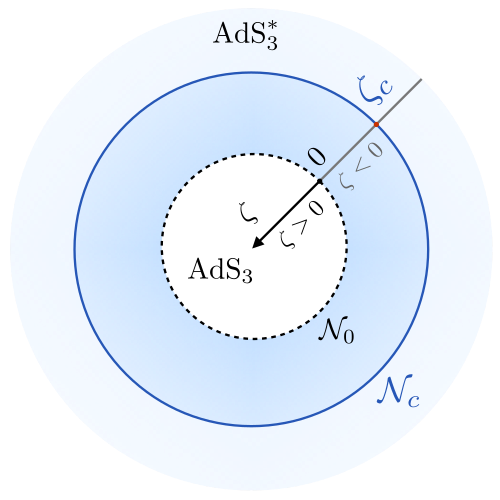
\includegraphics[width=\linewidth]{img/diagram.pdf}
	\vspace{-1.5\baselineskip}
	\caption{Glue-on $\mrm{AdS}_3$}
	
	\vspace{-.3\baselineskip}
	\scriptsize\ Top-down view of the Poincar\'e disk
\end{figure}
\end{column}
}

\begin{frame}{Glue-on $\mrm{AdS}_3$ / \TTbar --- updating the dictionary}{%
	\textcite{Apolo:2023vnm} -- \citetitle{Apolo:2023vnm}
}
\begin{columns}
\figGlueon
\begin{column}{.64\textwidth}
\vspace{-\baselineskip}
\begin{equation}
	\frac{1}{\zeta} \equiv \ell^{-2} g_{\varphi\varphi} \in \mbb{R},
\ \quad
	\zeta_c = - \frac{c \mu}{3\ell^2} \in \mbb{R}
\end{equation}
\vspace{-.5\baselineskip}
\begin{itemize}
\item What have we done other than copy-pasting?
	\begin{itemize}
	\item Although the continuation is straightforward, physical quantities diverge as $\rho \to 0$
	
	\item A prescription is required to ``renormalize'' the divergences
	\end{itemize}
	
\end{itemize}
\end{column}
\end{columns}
\end{frame}

\begin{frame}{Glue-on $\mrm{AdS}_3$ / \TTbar --- updating the dictionary}{%
	\textcite{Kraus:2018xrn} -- \citetitle{Kraus:2018xrn}
}
\begin{itemize}
\item Firstly, matching energy momentum (Brown-York) \& the flow equations:
	\begin{equation}
		T_{ij}= \frac{\sigma_{\zeta_c}}{8\pi G} \Big( K_{ij} -  K \gamma_{ij} + \frac{1}{\ell |\zeta_c|}\gamma_{ij}\Big), \ \quad \sigma_{\zeta_c} = \frac{\abs{\zeta_c}}{\zeta_c} = \pm 1,
		\label{BYtensor}
	\end{equation}
	The field theory metric $\gamma_{ij} = \zeta_c h_{ij}$, where $h_{ij}$ is the induced metric.
	
	\pause
	
	\begin{itemize}
	\item $\gamma_{ij}$ is always positive-definite, while $h_{ij}$ becomes negative-definite for the glue-on region.
	This discrepancy is the origin of the $\abs{\zeta_c}$.
	\end{itemize}
	
	\pause
	
\item \TTbar flow is recast geometrically as the $i,j$ components of the Einstein equations. 
Note that the geometry can be decomposed such that:
	\begin{equation}
		ds^2 = \frac{1}{\zeta} \gamma_{ij}dx^i dx^j+n_\mu n_\nu dx^\mu dx^\nu
	\end{equation}
\end{itemize}
\end{frame}


\begin{frame}{Glue-on $\mrm{AdS}_3$ --- beyond the infinity}{%
	\textcite{Apolo:2023vnm} -- \citetitle{Apolo:2023vnm}
}
\begin{itemize}
\item The geometry is foliated by constant $\zeta$ surfaces ${\mathcal N}_\zeta$:
	\begin{equation}
	\begin{aligned}
		ds^2 
		&= \ell^2 \bigg( \frac{d\rho^2}{4 \rho^2} + \frac{ \big( du + \rho \, \mathcal {\bar L}(v)\, dv \big) \big( dv + \rho \, \mathcal L(u)\, du \big) }{\rho} \bigg) \\
		&= \frac{1}{\zeta} \gamma_{ij}dx^i dx^j+n_\mu n_\nu dx^\mu dx^\nu,\ \quad
	\frac{1}{\zeta} \equiv \ell^{-2} g_{\varphi\varphi}
	\end{aligned}
	\end{equation}
	The \TTbar deformed theory lives on $\mcal{N}_{\zeta_c}$ with metric $\gamma_{ij}$.
	
\pause
\item Treatment for the singularity at $\zeta\to 0^\pm$: introduce $\mathcal N_{\zeta={\pm\epsilon}}$ and glue them together (``glue-on'');
	exclude the $-\epsilon < \zeta < \epsilon$ region until finally sending $\epsilon \to 0$. 
\item We formally denote the boundary surface by the limit $\mathcal N_{0}=\mathcal N_{0^+}=\mathcal N_{0^-}$, though we need to keep track of the asymptotic cutoff $\epsilon$ in actual computations.
\end{itemize}
\end{frame}

\newcommand{\stateGlueon}{\ensuremath{
	\textrm{Cutoff / \textit{glue-on} $\mrm{AdS}_{d+1}$ Gravity}
	\ \equiv\ %
	\textrm{\TTbar deformed $\mrm{CFT}_{d}$ at $\mcal{N}_{\zeta_c}$}\ \,
}}

\begin{frame}{Glue-on $\mrm{AdS}_3$ / \TTbar --- the proposal}{%
	\textcite{Apolo:2023vnm} -- \citetitle{Apolo:2023vnm}
}
\centering
\vspace{-.5\baselineskip}
\begin{minipage}{.5\textwidth}
\centering
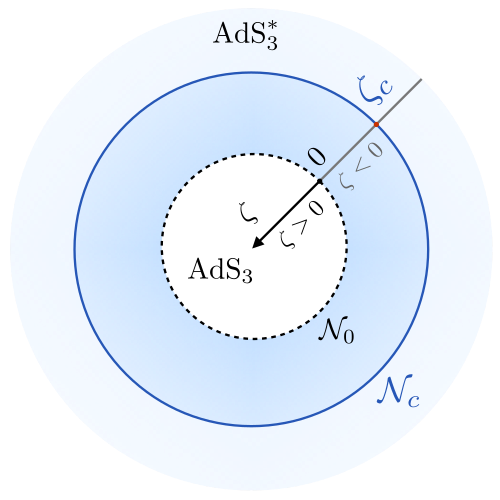
\includegraphics[width=.9\linewidth]{img/diagram.pdf}
\end{minipage}
\vspace{-.1\baselineskip}
\begin{equation*}
\stateGlueon
\end{equation*}
\end{frame}

\section{\textbf{Check:} \TTbar deformed charges \& partition functions} \label{se:charges}

\begin{frame}{\TTbar quantities from bulk geometry}{%
	\textcite{Apolo:2023vnm} -- \citetitle{Apolo:2023vnm}
}
\begin{columns}
\figGlueon[.3]
\begin{column}{.75\textwidth}
\begin{itemize}
\item AdS/CFT: weak / strong duality
	\begin{itemize}
	\item \textit{quantum} quantities on the CFT side\\
		can be computed by (semi-)classical geometry
	\item inherited by the \TTbar deformation
	\end{itemize}
	
\pause
\item Demanding the extended geometry to be non-singular
	re-produces bounds on the \TTbar deformed theory, e.g.
	\begin{equation}
		\zeta_c \ge -1 \quad \Leftrightarrow \quad\mu\le \frac{ 3\ell^2 }{c} \label{reality}
	\end{equation}
	$\zeta_c = -1$ is a horizon of the glue-on geometry, \\
	where $\det g_{\mu\nu} = 0$.
	
\end{itemize}
\end{column}
\end{columns}
\end{frame}


\begin{frame}{\TTbar spectrum from bulk covariant charges}{%
	\textcite{Kraus:2021cwf,Apolo:2023vnm}
}
\begin{columns}
\figGlueon[.3]
\begin{column}{.75\textwidth}
\vspace{-.3\baselineskip}
\begin{itemize}
\item Spectrum: conserved charges of geometries,\\
	e.g.~black holes \textit{BTZ} \cite{Banados:1992wn}
	\begin{itemize}
	\item computed with the covariant formalism\\
		\textcite{Iyer:1994ys, Barnich:2001jy}
	\item manifest covariance (diff-invariance) depends on reparametrization redundancies (gauge),\\
		so delay gauge fixing until the very end
	\end{itemize}
	
\pause
\item We are careful to match the bulk \& boundary symmetries at $\mcal{N}_{\zeta_c}$

\item This reproduces $E(\mu)$, $J(\mu)$ with $\mu \in\mbb{R}$ in \eqref{ttbarspectrum}
	
\end{itemize}
\end{column}
\end{columns}
\end{frame}


\begin{frame}{\TTbar spectrum from bulk covariant charges}{%
	\textcite{Kraus:2021cwf,Apolo:2023vnm}
}
\begin{columns}
%\figGlueon[.3]
\begin{column}{\textwidth}
\vspace{-.3\baselineskip}
\begin{itemize}
\item Covariant charges of geometries
	\begin{align*}
		\delta E(\mu) &\equiv  \ell^{-1} \delta \mathcal Q_{\pd_{t'}}, \\ \delta J(\mu) &\equiv  \delta \mathcal Q_{\pd_{\varphi'}},
	\end{align*}

\item One needs to choose the appropriate boundary coordinates $(t',\varphi')$, such that
	\begin{equation}
		ds^2_c = \ell^2 ( -dt'^2 + d\varphi'^2) , \qquad \varphi' \sim \varphi' + 2\pi.\label{cutoffmetric}
	\end{equation}

\pause

\item This is realized by the \textit{state-dependent} map of coordinates
	\begin{align*}
		dt' &= \sqrt{ \big(1 - \zeta_c (T_u+T_v)^2 \big) \big(1 - \zeta_c (T_u-T_v)^2 \big) } \, dt,  \\
		 d\varphi' &= d\varphi + \zeta_c \big( T_u^2 - T_v^2 \big)\,dt.
	\end{align*}
\end{itemize}
\end{column}
\end{columns}
\end{frame}

\begin{frame}{\TTbar thermodynamics from bulk geometry}{%
	\textcite{Giveon:2017nie,Apolo:2019zai}
}
\begin{columns}
%\figGlueon[.3]
\begin{column}{\textwidth}
\vspace{-.3\baselineskip}
\begin{itemize}

\item \textit{State-dependent} map of coordinates
	\begin{align*}
		dt' &= \sqrt{ \big(1 - \zeta_c (T_u+T_v)^2 \big) \big(1 - \zeta_c (T_u-T_v)^2 \big) } \, dt, \\
		 d\varphi' &= d\varphi + \zeta_c \big( T_u^2 - T_v^2 \big)\,dt.
	\end{align*}

\pause
\item Many consequences: correct charges, signal propagation speed $v'_{\pm} \equiv \pm \frac{d\varphi'}{dt'}$, and thermodynamics when Wick rotated:
	\begin{equation}
		T_L(\mu)\,T_R(\mu) \le - \frac{1}{4\pi^2 \ell^2 \zeta_c} = \frac{3}{4\pi^2c\mu} = T_H(\mu)^2,
	\quad \mu > 0
	\end{equation}
	$T_{L,R}$ are temperatures associated with $u',v' = \varphi' \pm t'$.

\item $T_H$ is the \textit{Hagedorn temperature}: exceeding $T_H$ corresponds to a complex entropy
\end{itemize}
\end{column}
\end{columns}
\end{frame}

\section{\textbf{Check:} \TTbar partition functions from glue-on AdS} \label{se:partitionfunction}

\begin{frame}{\TTbar partition functions from bulk on-shell actions}{%
	\textcite{Caputa:2020lpa}
}
\begin{columns}
\figGlueon
\hspace{-1.5em}
\begin{column}{.7\textwidth}
\vspace{-.3\baselineskip}
\begin{itemize}
\item Bulk: weakly coupled gravity, the partition function is approximated by the on-shell gravity action of the dominant saddle:
	\begin{equation}
		Z_{T\bar T} (\mu) = \mathcal Z (\zeta_c) \approx  e^{-I(\zeta_c)}\label{partition2}
	\end{equation}

\pause
\item $I(\zeta_c)$ is roughly the volume of the geometry, which diverges at $\zeta \to 0^\pm$. We apply a natural extension of \textit{holographic renormalization} to remove the divergence.

\pause
\item $I = -\log \mcal{Z}$ satisfies the \TTbar flow \eqref{TTbardef}.\\
	This is non-trivial because we've packaged the quantum corrections of the boundary theory.
\end{itemize}
\end{column}
\end{columns}
\end{frame}

\begin{frame}{Comparison with field theory analysis}{%
	\textcite{Datta:2018thy,Apolo:2023aho}
}
\begin{columns}
%\figGlueon
%\hspace{-1.5em}
\begin{column}{\textwidth}
\vspace{-.3\baselineskip}
\begin{itemize}
\item \textbf{Torus:} Large $c$, \textit{modular invariance} \& sparseness of the ``light'' spectrum \cite{Datta:2018thy,Apolo:2023aho},
	c.f. \textcite{Hartman:2014oaa}
	\begin{equation*}
	\hspace{-1.5em}
		\log   Z_{T\bar T}(\mu)  \approx \left\{ \begin{aligned}
		& {-\frac{1}{2}}\,(\beta_L + \beta_R)\, RE_{\text{vac}}(\mu),  &\beta_L \beta_R > 1, \\
		& {-2 \pi^2 \bigg(\frac{1}{\beta_L} + \frac{1}{\beta_R}\bigg)  RE_{\text{vac}}\bigg(\frac{4\pi^2}{\beta_L \beta_R} \mu \bigg)}, \ \, &\beta_L\beta_R < 1, %\\[2ex]
		 \end{aligned} \right. %\label{ZTTbar}
	\end{equation*}
	
\item \textbf{Sphere:} maximally symmetric, \textcite{Donnelly:2018bef}
	\begin{equation}
%		\label{sphere:stresstensor}
		\langle T_{ij}\rangle =-\frac{1}{4\pi\mu} \bigg(1-\sqrt{1-\frac{c\mu}{3L^2}}\, \bigg)  \gamma_{ij}.
	\end{equation}
\end{itemize}
\end{column}
\end{columns}
\end{frame}

\begin{frame}{Sphere partition functions}{%
	\textcite{Donnelly:2018bef,Li:2020zjb}
}
\begin{columns}
%\figGlueon
%\hspace{-1.5em}
\begin{column}{\textwidth}
\vspace{-.3\baselineskip}
\begin{itemize}

\item Given the explicit stress tensor $\langle T_{ij}\rangle \propto \gamma_{ij}$, the flow equations:
	\begin{align*}
\partial_\mu \log Z_{\TTbar}(\mu)&=8\pi \int d^2x\sqrt{\gamma}\, \langle T\bar{T} \rangle \\
-L\,\partial_L \log Z_{\TTbar}(\mu)&=\int d^2x\sqrt{\gamma}\,\langle T^i_i \rangle
	\end{align*}

	\item ... admit the general solution with a $\mu$-\textit{independent} integration $a$:
	\begin{equation*}
		\log Z_{\TTbar}(\mu, a) = \frac{c}{3} \log \bigg[\frac{L}{a}   \bigg(1+\sqrt{1-\frac{c \mu }{3  L^2}}\, \bigg) \bigg] - \frac{L^2}{\mu}  \sqrt{1-\frac{c \mu }{3 L^2}} + \frac{L^2}{\mu} %\label{Zsol}
	\end{equation*}

	\item \textcite{Donnelly:2018bef} is recovered with $a = \sqrt{c|\mu|/3}$ but one can also take $a = \epsilon$, thus decoupling the energy (RG) scale $\epsilon$ with the deformation $\mu$. 
\end{itemize}
\end{column}
\end{columns}
\end{frame}

\begin{frame}{Gravitational actions: with counterterms}{%
	\textcite{Donnelly:2018bef,Li:2020zjb}
}
\begin{columns}
%\figGlueon
%\hspace{-1.5em}
\begin{column}{1.1\textwidth}
\vspace{-.3\baselineskip}
\begin{itemize}

\item Gravitational actions, with counterterms:
	\begin{align*}
		I_{\mcal{M}}(\zeta_1, \zeta_2) & \coloneqq - \frac{1}{16\pi G} \int_{\zeta_1}^{\zeta_2} d\zeta \int d^2 x \sqrt{g} \, (R + 2 \ell^{-2}),  %\label{bulkaction} \\
	\\
		I_{\mathcal N_{\zeta}} & \coloneqq  - \frac{1}{8\pi G} \int_{\mathcal N_{\zeta}} d^2x \sqrt{h}\,h^{ij} K_{ij} 
	\\& \qquad + \frac{\sigma_\zeta}{8\pi G} \int_{\mathcal N_{\zeta}} d^2x \sqrt{h} \, \bigg(\ell^{-1} - \frac{\ell  \mathcal{R}[h]}{4} \log |\zeta| \bigg), %\label{boundaryaction}
	\end{align*}
	... consistent with the Brown-York stress tensor $T_{ij}$, \\
	fully renormalized at $\zeta \to 0^\pm$. 
	
	\item The lack of diff invariance of the $\log |\zeta|$ counterterm is known to be a reflection of the Weyl anomaly: \textsl{\citeauthor{Henningson:1998gx,deHaro:2000vlm,Papadimitriou:2010as}}.
	
\end{itemize}
\end{column}
\end{columns}
\end{frame}

\begin{frame}{Gravitational actions: with counterterms}{%
	\textcite{Caputa:2020lpa,Li:2020zjb}
}
\begin{columns}
%\figGlueon
%\hspace{-1.5em}
\begin{column}{1.1\textwidth}
\vspace{-.3\baselineskip}
\begin{itemize}

\item The $\log$ counterterm makes a crucial contribution to the on-shell action:
	\begin{align*}
		I_{\mcal{M}}(\zeta_1, \zeta_2) & \coloneqq - \frac{1}{16\pi G} \int_{\zeta_1}^{\zeta_2} d\zeta \int d^2 x \sqrt{g} \, (R + 2 \ell^{-2}),  %\label{bulkaction} \\
	\\
		I_{\mathcal N_{\zeta}} & \coloneqq  - \frac{1}{8\pi G} \int_{\mathcal N_{\zeta}} d^2x \sqrt{h}\,h^{ij} K_{ij} 
	\\& \qquad + \frac{\sigma_\zeta}{8\pi G} \int_{\mathcal N_{\zeta}} d^2x \sqrt{h} \, \bigg(\ell^{-1} - \frac{\ell  \mathcal{R}[h]}{4} \log |\zeta| \bigg), %\label{boundaryaction}
	\end{align*}
	It guarantees that the partition function is compatible with the $T\bar T$ differential equation --- not the case for \textsl{\citeauthor{Donnelly:2018bef}}.
	
	\item In general the space of deformed theories are parametrized by $(\mu,a)$, where $a$ is the length scale (inverse energy scale). In many contexts they are naturally related: $a = \sqrt{c|\mu|/3}$, but $a$ can be tuned by RG.
	
\end{itemize}
\end{column}
\end{columns}
\end{frame}


\section{Summary \& future directions}

\begin{frame}{Glue-on $\mrm{AdS}_3$ / \TTbar deformed $\mrm{CFT}_2$}{%
	\textcite{Apolo:2023vnm} -- \citetitle{Apolo:2023vnm}
}
\vspace{-2\baselineskip}
\begin{equation*}
\stateGlueon
\end{equation*}
\vspace{-1.3\baselineskip}
\begin{columns}
\begin{column}{.37\textwidth}
\begin{figure}[!h]
	\centering
	\includegraphics[width=\linewidth]{img/RT-AdS.pdf}
	\vspace{-1.5\baselineskip}
	\caption{RT for Glue-on $\mrm{AdS}_3$}
	
	\vspace{-.3\baselineskip}
	\scriptsize\, Top-down view of the Poincar\'e disk
\end{figure}
\end{column}
\hspace{-1em}
\begin{column}{.71\textwidth}
\begin{itemize}
\item Holographic proposal for $T\bar T$-deformed CFTs\\
with $\mu \in \mbb{R}$.

\item As evidence, we show that the $T\bar T$ trace flow equation, the spectrum on the cylinder, and the partition function on the torus and the sphere, among other results, can all be reproduced from bulk calculations in glue-on AdS$_3$.

\pause
\item We hope to understand the entanglement structure of \TTbar deformed theories from bulk geometry. 
\end{itemize}
\end{column}
\end{columns}
\end{frame}


\begin{frame}{Glue-on $\mrm{AdS}_3$ / \TTbar deformed $\mrm{CFT}_2$}{%
	\textcite{Apolo:2023vnm} -- \citetitle{Apolo:2023vnm}
}
\vspace{-2\baselineskip}
\begin{equation*}
\stateGlueon
\end{equation*}
\vspace{-1.3\baselineskip}
\begin{columns}
\begin{column}{.37\textwidth}
\begin{figure}[!h]
	\centering
	\includegraphics[width=\linewidth]{img/RT-AdS.pdf}
	\vspace{-1.5\baselineskip}
	\caption{RT for Glue-on $\mrm{AdS}_3$}
	
	\vspace{-.3\baselineskip}
	\scriptsize\, Top-down view of the Poincar\'e disk
\end{figure}
\end{column}
\hspace{-1em}
\begin{column}{.71\textwidth}
\begin{itemize}

\item We hope to understand the entanglement structure of \TTbar deformed theories from bulk geometry. \pause
	\begin{itemize}
	\item \textcite{Donnelly:2018bef,Lewkowycz:2019xse}
	\item \textcite{He:2023xnb,He:2023wko,Tian:2023fgf,Hou:2023ytl}
	\end{itemize}
\end{itemize}
\end{column}
\end{columns}
\end{frame}

\begin{frame}

\centering

\huge
\sidenote{Thank you!}
\bigskip

\large
froms Wen-Xin Lai\ \textkai{赖文昕}

\textit{\normalsize in collaboration with}

	Luis Apolo,
	Peng-Xiang Hao \textkai{郝鹏翔}
	and Wei Song \textkai{宋伟}\\[2ex]
\sidenote{\arxiv{2303.04836}}
%\ submitted to \textit{JHEP}

\end{frame}




\begin{frame}[allowframebreaks]{References}
\renewcommand*{\bibfont}{\footnotesize}
\printbibliography %%% should not specify heading etc
\end{frame}


\end{document}
